% please use TexLive 2014 or later with the M&C macros freely
% available from tug.org or use any other recent version of LaTeX

\documentclass{article}\usepackage[]{graphicx}\usepackage[table]{xcolor}
% maxwidth is the original width if it is less than linewidth
% otherwise use linewidth (to make sure the graphics do not exceed the margin)
\makeatletter
\def\maxwidth{ %
  \ifdim\Gin@nat@width>\linewidth
    \linewidth
  \else
    \Gin@nat@width
  \fi
}
\makeatother

\definecolor{fgcolor}{rgb}{0.345, 0.345, 0.345}
\newcommand{\hlnum}[1]{\textcolor[rgb]{0.686,0.059,0.569}{#1}}%
\newcommand{\hlstr}[1]{\textcolor[rgb]{0.192,0.494,0.8}{#1}}%
\newcommand{\hlcom}[1]{\textcolor[rgb]{0.678,0.584,0.686}{\textit{#1}}}%
\newcommand{\hlopt}[1]{\textcolor[rgb]{0,0,0}{#1}}%
\newcommand{\hlstd}[1]{\textcolor[rgb]{0.345,0.345,0.345}{#1}}%
\newcommand{\hlkwa}[1]{\textcolor[rgb]{0.161,0.373,0.58}{\textbf{#1}}}%
\newcommand{\hlkwb}[1]{\textcolor[rgb]{0.69,0.353,0.396}{#1}}%
\newcommand{\hlkwc}[1]{\textcolor[rgb]{0.333,0.667,0.333}{#1}}%
\newcommand{\hlkwd}[1]{\textcolor[rgb]{0.737,0.353,0.396}{\textbf{#1}}}%
\let\hlipl\hlkwb

\usepackage{framed}
\makeatletter
\newenvironment{kframe}{%
 \def\at@end@of@kframe{}%
 \ifinner\ifhmode%
  \def\at@end@of@kframe{\end{minipage}}%
  \begin{minipage}{\columnwidth}%
 \fi\fi%
 \def\FrameCommand##1{\hskip\@totalleftmargin \hskip-\fboxsep
 \colorbox{shadecolor}{##1}\hskip-\fboxsep
     % There is no \\@totalrightmargin, so:
     \hskip-\linewidth \hskip-\@totalleftmargin \hskip\columnwidth}%
 \MakeFramed {\advance\hsize-\width
   \@totalleftmargin\z@ \linewidth\hsize
   \@setminipage}}%
 {\par\unskip\endMakeFramed%
 \at@end@of@kframe}
\makeatother

\definecolor{shadecolor}{rgb}{.97, .97, .97}
\definecolor{messagecolor}{rgb}{0, 0, 0}
\definecolor{warningcolor}{rgb}{1, 0, 1}
\definecolor{errorcolor}{rgb}{1, 0, 0}
\newenvironment{knitrout}{}{} % an empty environment to be redefined in TeX

\usepackage{alltt}

%the main style; default LibreCaslon font
% \usepackage[raggedsec,sectionbib]{morgan2}
% \usepackage{morgan-defs}

%to use Times New Roman, instead of LibreCaslon, please uncomment the next line
%\morgansetup{fontsetup=times}

% bibliography
% \usepackage[comma,sort,authoryear]{natbib}         % author-year
\usepackage[square,comma,sort&compress,numbers]{natbib} % numbered
% \usepackage{makeidx}     % Per Tondo's suggestion on 1 Feb 2022.
% \usepackage{chapterbib}

% 
% Begin LaTeX packages imported by the authors.
% 

% \usepackage{booktabs}    % For awesome table formatting
\usepackage{caption}     % Necessary for the subcaption package?
% \usepackage{epigraph}    % For epigraphs below chapter titles.
\usepackage{eurosym}     % For the EU currency symbol.
\usepackage{gensymb}     % For the \degree command.
\usepackage{microtype}   % For (more) beautiful typesetting.
\usepackage{rotating}    % For rotating figures.
\usepackage[normalem]{ulem} % For strikethrough text.
\usepackage{subcaption}  % For labeling subfigures.
\usepackage{tikz}
\usetikzlibrary{arrows}
\usetikzlibrary{positioning}
\usetikzlibrary{shapes.geometric}
\usepackage{wrapfig}     % To wrap text around figures.
\usepackage[table]{xcolor}      % makes colored text.

% The morgan-defs.sty file already loads the enumitem package.
% Add the inline option here
% for inline enumerate* lists.
% \PassOptionsToPackage{inline}{enumitem}

% 
% Begin LaTeX macros created by the authors.
% 

% Temperatures
\newcommand{\degC}{\degree C}
\newcommand{\degF}{\degree F}
% Figure widths
\newcommand{\figwidth}{0.85\linewidth}
% The "math font trick" to get Libre Caslon font in italics inside equations.
\newcommand{\mft}[1]{\text{\emph{#1}}}
\newcommand{\ICOtwonodollar}{\mft{I}_{\text{CO}_2}}
\newcommand{\ICOtwo}{$\ICOtwonodollar{}$}
\newcommand{\ICOtwoparen}{(\ICOtwo{})}
\newcommand{\Iparen}{(\:\!\mft{I}\:\!)}
\newcommand{\Pparen}{(\:\!\mft{P}\;\!)}
\newcommand{\Aparen}{(\;\!\mft{A}\:\!)}
\newcommand{\Rparen}{(\:\!\mft{R}\;\!)}
\newcommand{\REpnodollar}{\mft{R}_{\mft{Ep}}}
\newcommand{\REp}{$\REpnodollar$}
\newcommand{\REpparen}{(\:\!\REp)}
\newcommand{\Xparen}{(\;\!\mft{X}\:)}
\newcommand{\XCOtwonodollar}{\mft{X}_{\text{CO}_2}}
\newcommand{\XCOtwo}{$\XCOtwonodollar$}
\newcommand{\XCOtwoparen}{(\;\!\XCOtwo)}
\newcommand{\Tparen}{(\mft{T}\:)}

\newcommand{\rateICOtwo}{$\mft{r}_{\ICOtwonodollar{}}$}
\newcommand{\rateP}{$\mft{r}_{\mft{P}}$}
\newcommand{\rateA}{$\mft{r}_{\mft{A}}$}
\newcommand{\rateREp}{$\mft{r}_{\REpnodollar{}}$}
\newcommand{\rateXCOtwo}{$\mft{r}_{\XCOtwonodollar{}}$}


% IPARX equation
\newcommand{\iparx}{
\footnotesize
\begin{tabular}{ccccccccc}
\mft{I}  & = & \mft{P}        & $\times$ & \mft{A}       & $\times$ & \mft{R}      & $\times$ & \mft{X} \\
\multirow{2}{*}{Impact} &  & \multirow{2}{*}{Population} &  & \multirow{2}{*}{Affluence} &  & Resource intensity &  & Impact \\
 &  &  &  &  &  & of the economy &  & of resources \\
$\left[\frac{\text{impact}}{\text{year}}\right]$ & & $\left[\text{persons}\right]$ &  & $\left[\frac{\text{\$ GDP}}{\text{person$\cdot$year}}\right]$ &  & $\left[\frac{\text{resources}}{\text{\$ GDP}}\right]$ &  & $\left[\frac{\text{impact}}{\text{resources}}\right]$
\end{tabular}
\normalsize
}


%
% Create environments for questions and projects, 
% as suggested by Tondo on 14 July 2021.
%

\newenvironment{questions}%
{\begin{enumerate}
\renewcommand{\labelenumi}{Q\thechapter.\arabic{enumi}}
\renewcommand{\theenumi}{Q\thechapter.\arabic{enumi}}}
{\end{enumerate}}

\newenvironment{projects}%
{\begin{enumerate}
\renewcommand{\labelenumi}{P\thechapter.\arabic{enumi}}
\renewcommand{\theenumi}{P\thechapter.\arabic{enumi}}}
{\end{enumerate}}


%
% End author additions
% 


\setcounter{secnumdepth}{2}

\graphicspath{{./figures/}}     % folder for the figures in your book

\PassOptionsToPackage{hyphens}{url}
\usepackage[colorlinks=true,linkcolor=MyDarkBlue,
citecolor=MyDarkBlue,filecolor=MyDarkBlue,urlcolor=MyDarkBlue]{hyperref}
\usepackage{doi}

\renewcommand{\UrlBreaks}{\do\.\do\@\do\\\do\/\do\!\do\_\do\|\do\;\do\>\do\]%
\do\)\do\,\do\?\do\&\do\'\do+\do\=\do\#%
\do\a\do\b\do\c\do\d\do\e\do\f\do\g\do\h\do\i\do\j%
\do\k\do\l\do\m\do\n\do\o\do\p\do\q\do\r\do\s\do\t%
\do\u\do\v\do\w\do\x\do\y\do\z\do\A\do\B\do\C\do\D%
\do\E\do\F\do\G\do\H\do\I\do\J\do\K\do\L\do\M\do\N%
\do\O\do\P\do\Q\do\R\do\S\do\T\do\U\do\V\do\W\do\X%
\do\Y\do\Z}
\makeatletter
\g@addto@macro{\UrlBreaks}{\UrlOrds}
% \renewcommand{\ALG@name}{\color{black}Algorithm}
\makeatother
\IfFileExists{upquote.sty}{\usepackage{upquote}}{}
\begin{document}

\title{A Calvin Core 100 Introduction to Sustainability}
\author{Jeremy Van~Antwerp, Matthew Kuperus Heun}

% \mainmatter
 
Let’s begin with a story.
Once upon a time, a king was challenged to a game of chess by a poor scholar.
If he lost, the king would have to pay the scholar a chessboard’s worth of
grain, defined as one kernel of grain on the first square, two grains on the second
square, four grains on the third square, and so on, with each subsequent square receiving
double what was on the previous square.
The king accepted the wager but lost the game.
A chessboard
has eight rows and eight columns, so the king had to pay 2$^\text{64}-$1
grains.
(See Section \ref{sec:exp} for an explanation of the math behind this formula.)
Rice is 7,000 grains per pound ($\sim$~65~mg each),
so the king owed the scholar 1.199~$\times$~10$^{\text{15}}$ kg of rice,
which is more than 150 tons of rice for every person currently on planet Earth
(worth about \$40,000 per person).
For reference, people eat about 35 tons of food in a lifetime,
so this is~4.4 lifetimes' supply of food for every person on the planet.
Clearly, the scholar's winnings won't all fit on an ordinary chessboard!

This story, which goes back at least to the 1200s AD, illustrates several aspects of the
sustainability problem that have been evident for centuries:
\textbf{Exponential growth} (Section \ref{sec:exp}) is
inherently not sustainable;
big numbers are hard to \href{https://en.wiktionary.org/wiki/grok}{grok};
and making large wagers on limited understanding is unwise.
At the moment, human society is making the king's wager writ large.
We are pursuing exponential growth without fully understanding the consequences.
In short, we have \textbf{sustainability challenges}.

You are reading this book because you think sustainability is important.
And it is.
In the long run, sustainability is one of the few things that matter at all.
Sustainability is a challenging problem, in part due to exponential growth,
in part due to limited understanding,
but also because sustainability problems are complex and interconnected.
Each of the subproblems or subdomains of sustainability may have its own problems
of exponential growth and limited knowledge.

Furthermore, the king's wager hints at a social element of the sustainability problem.
In the story, the king doesn't want to appear ``weak'' before his subject and so
(rashly) accepts the wager.
In sustainability, there is tremendous social (and sometimes economic) pressure
to continue to do things ``the way they've always been done.''

Figure~\ref{fig:venn_diagram} shows the three interrelated and overlapping domains
of sustainability:
\textbf{environmental sustainability},
\textbf{economic sustainability}, and
\textbf{social sustainability}.
Sustainability problems are complex and interconnected.
Environmental sustainability problems have social and economic aspects (that are
generally more difficult to solve).
Likewise, economic and social sustainability problems are not limited to one domain;
typically, they include aspects of the other two domains as well.
Therefore (for example), pollution is an environmental problem, and a social problem, and an economic problem.
Likewise renewable energy. And land use. And all the other challenges humanity faces.

\begin{figure}
\centering

  % The next command tells RStudio to do "Compile PDF" on book.Rnw,
% instead of this chapter, thereby eliminating the need to switch back to book.Rnw 
% before making the book.
%!TEX root = ../../book.Rnw

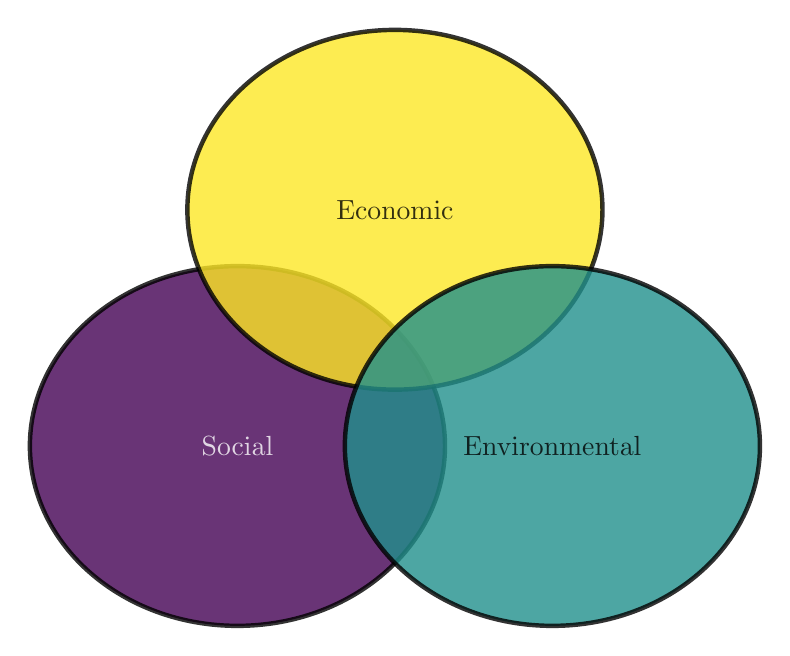
\begin{tikzpicture}
    \definecolor{my_purple}{HTML}{440154}
    \definecolor{my_yellow}{HTML}{FDE725}
    \definecolor{my_green}{HTML}{21908C}
    \tikzstyle{every node}=[ultra thick, ellipse, 
                            minimum width = 150pt,
                            minimum height = 130pt]
    \node[ellipse, draw, fill = my_purple, opacity = 0.8, align = left, text = white] (social) at (-2,0) {Social};
    \node[ellipse, draw, fill = my_yellow, opacity = 0.8, align = center] (economic) at (0,3) {Economic};
    \node[ellipse, draw, fill = my_green, opacity = 0.8, align = right] (environmental) at (2,0) {Environmental};
\end{tikzpicture}


  \caption[Three aspects of sustainability]
          {The three aspects of sustainability.
           Sustainability is often visualized as three overlapping ellipses:
           economic sustainability,
           environmental sustainability, and
           social sustainability.
           The intersecting area represents fully sustainable living.
           Environmental sustainability
           refers to the \textbf{ecosystem} and its supporting services.
           Economic sustainability
           refers to human systems for creating and accounting for wealth;
           see Chapter~\ref{chap:affluence}.
           Social sustainability
           refers to traditions and systems of human society.
           The layering in this figure represents coverage in this book.
           We focus on environmental and
           economic sustainability.
           Social sustainability is vitally important, so it forms the backdrop
           for much of the discussion herein.}
\label{fig:venn_diagram}
\end{figure}


Sustainability is challenging for two additional reasons.
First, it may seem that the changes required to achieve sustainability are so
massively overwhelming that they shouldn't even be addressed.
Second, it may seem like the consequences of not becoming sustainable are so far
in the future that there is neither urgency nor immediate payback.
However, neither of these views is true.
Current news headlines indicate that we are already
experiencing the effects of not being sustainable, in all
sustainability domains---environmentally, economically, and socially.
There are many reasonable and simple things that can be done to improve our
sustainability in the near term.
The deep changes needed for long-term sustainability are urgently needed precisely because
they are long-term investments.
The sooner we begin making those investments, the sooner we'll begin reaping the
rewards and the greater those rewards will be.


%%%%%%%%%%%%%%%%%%%%%%%%%%%%%%%%%%%%%%%%%%%%%%%%%%%%%%%%%%%%%%
\section{Purpose and focus}
%%%%%%%%%%%%%%%%%%%%%%%%%%%%%%%%%%%%%%%%%%%%%%%%%%%%%%%%%%%%%%

This book summarizes ways that humans are not living sustainably and suggests
characteristics of sustainable societies.
The text is deliberately short because the book is not intended to be comprehensive.
The focus is on equipping the reader to discuss moral and ethical issues around sustainability.
Because the choices and paths to sustainability are filled with value judgments and moral choices,
the end-of-chapter discussion questions mostly point to tradeoffs and do not have ``right answers.''
Instead, different answers indicate different preferences.
This book presents a coherent framework for discussing sustainability
that is grounded in a sense of scale.
Therefore, we prioritize presenting information graphically.
The intent is to equip readers with basic knowledge (informed by scale) so we can
grapple with tough moral questions.
\emph{This book should be easy to read but hard to digest.}
As you read this book, it should raise many questions for you.

The focus of this book is the many challenges of sustainability.
While we may, at times, point to directions for improved sustainability
(Chapters~\ref{chap:government} and~\ref{chap:personal_action}),
it is beyond our scope
(and indeed our ability) to provide solutions for all sustainability problems.
Some (or many) of the questions that are raised about sustainability
will remain unanswered.

Our framework for describing sustainability challenges
is illustrated by data.
Thus, readers can expect graphs, tables, and other numerical representations
of the state of our world as it relates to sustainability.
Part~\ref{part:IPARX} (Chapters~\ref{chap:introduction}--\ref{chap:impact_intensity})
shows mostly data from the world in aggregate, thereby eliminating issues of
imports and exports between countries.
Part~\ref{part:sustainability_challenges} shows data mostly from the U.S.%
\footnote{
  Readers are encouraged to remember that the U.S.\ is atypical in many ways.
  Sociologically, the U.S.\ is WIERD
    (Western, industrialized, educated, rich, and democratic).
  Additionally, the U.S.\ has a low population density
  and lots of resources.
  While our framework for sustainability thinking is universal, the data used for
  illustration may not always apply to the rest of the world.
},
because it is our home country and
because it has better data coverage than most countries
regarding energy and carbon emissions.
Behind the facts and data are important concepts related to human choices,
which we explore throughout the book, mostly in questions and projects that follow each chapter.

The remainder of this chapter summarizes key themes of the book.


%%%%%%%%%%%%%%%%%%%%%%%%%%%%%%%%%%%%%%%%%%%%%%%%%%%%%%%%%%%%%%
\section{What is sustainability?}
\label{sec:what_is_sustainability}
%%%%%%%%%%%%%%%%%%%%%%%%%%%%%%%%%%%%%%%%%%%%%%%%%%%%%%%%%%%%%%

``Sustainability'' is a crucial concept.
If humanity is not living sustainably, we will either cease to exist as a species
or (at least) experience drastic reductions in our population and/or standard of living.
So, what is sustainability and how do we tell if we're living sustainably?
There are many definitions of sustainability.
To the novice, many definitions may seem to indicate lack of agreement.
However, sustainability is almost a self-defining concept.
Different answers indicate different assumptions, different priorities, and different
boundaries (that is, what system is being considered).

When considering the meaning of sustainability, the two most important questions are
``sustaining what?'' and ``for how long?''
The second of these questions is perhaps easier to answer.
Although humans seem to have inherent cognitive difficulties in planning for
time scales significantly longer than the human lifespan,
\textbf{strong sustainability} is achieved only if the answer is
``indefinitely'' or ``forever.''
Our current sustainability crisis has been thousands of years in the making~\cite{Sanderman2017}
and will likely require millions of years to recover~\cite{Davis11262}.
A \textbf{weak sustainability} criterion is sustainability over a long (by human standards)
time frame, perhaps 50 years, which is on the order of one human adulthood.%
\footnote{
  Our criteria for strong and weak sustainability are physical and
  follow \citet{Graedel:2010ab}.
  Other definitions for weak and strong sustainability exist.
  One approach to weak and strong sustainability is economic.
  It defines strong sustainability as protecting natural capital 
  for a certain period of time
  (equivalent to our weak sustainability definition 
  if the time horizon for protecting natural capital is 50 years).
  In the economic approach,
  weak sustainability allows 
  produced capital
  to substitute for natural capital
  across a period of time.
  See \citet{Dietz:2007tu} for details.
}
(Note that corporate time scales for decision making are even shorter,
often in the 5--20 year range; see Chapter~\ref{chap:government}.)

The narrowest answer for what needs sustaining is human life and society, which
\href{https://www.merriam-webster.com/dictionary/perforce}{perforce}
entails those \textbf{ecosystem services}
(Chapter~\ref{chap:planetary_boundaries})
necessary for human health and wellbeing.
Beyond these basics, some people view the nonhuman world as having inherent 
worth or standing and, therefore, to be worth preserving.
For some people, the inclination for preservation is limited to those parts
of the nonhuman world that humans find appealing, like flowers and songbirds.
Other people would include even those parts of the nonhuman world that negatively
affect humanity, like smallpox.
Unfortunately, humans don’t know clearly what pieces of the ecosystem
are, in the long run, necessary for our survival and which aren’t.
For instance, could we survive in a world without dandelions?
Maybe.
On the other hand, dandelions might be necessary for other organisms we depend on.
Environmental science views the ecosystem in its entirety as a web, with all parts
depending on all other parts.
The ecosystem is not a collection of individual components with binary ``needed''/``not
needed'' classifications, but as a whole that exists on a continuum from ``fully functional''
to ``nonfunctional.''
The choices and paths to sustainability are bristling with value judgments and
moral choices about what to value and how much.
\href{https://en.wiktionary.org/wiki/concomitant}{Concomitant} with such choices
is a weighting of appropriate risks to the ecosystem and human society.
Different answers to these questions come from different \emph{a priori} assumptions and values.

The broadest definitions of sustainability
also include the products of human civilization.
For example, although they are great cultural and historical artifacts,
humanity could survive without the great pyramids of Giza.
On the other hand, we may not survive if we don’t give up coal-fired power plants.
(And, maybe many people would perish if the coal-fired power plants
were all suddenly switched off.)

With respect to Figure \ref{fig:venn_diagram}, environmental sustainability
considers biophysical and thermodynamic constraints and includes issues such as
pollution, resource depletion, habitat loss, and biodiversity.
Harvesting timber faster than it can grow is unsustainable.
Eventually, deforestation means that timber harvesting must stop because there
will be no more forest to harvest.
Depleting \textbf{mineral resources} is unsustainable.
Eventually, the minerals will be used up.
Pumping \textbf{aquifers} faster than they can regenerate is unsustainable.
Eventually, the aquifers will run dry.

Economic sustainability
involves questions of profit and loss, wealth management, and
macroeconomic policy.
A business that continually loses money is not sustainable.
Eventually, it will go out of business.

Social sustainability comprises human and 
civil rights,
suffering, and personal freedom.
A social group that continually loses members, for example, the Whig party, will
cease to be a group.
Often, a discussion about social sustainability 
includes things that should not be sustained but that, typically, 
have persisted a very long time, 
like poverty, class inequality, sexism, slavery, and other civil injustices.

This book discusses issues associated with each of these three
sustainability domains but with a focus on energy and carbon emissions.
The end-of-chapter questions typically focus on interactions among the three
domains, like a social-vs.-economic tradeoff.

%^^^^^^^^^^^^^^^^^^^^^^^^^^^^^^
\begin{mcframe}[0.90\textwidth](0.85\textwidth)
%^^^^^^^^^^^^^^^^^^^^^^^^^^^^^^
This book uses energy and carbon emissions as prime examples not
because they are the only sustainability problems, but because
energy is the \textbf{master resource} and \textbf{climate change}
is currently one of the most urgent sustainability problems.
Energy and carbon emissions
link together many of our sustainability challenges.
\end{mcframe}

The most oft-quoted~\cite{Quental2011} definition of sustainability is that
\textbf{sustainable development} ``meets the needs of the present without
compromising the ability of future generations to meet their own needs''~\cite{Brundtland}.
Note that sustainable development is an oxymoron, %and is not the same as sustainability.
because ``development'' implies constant improvement, which cannot be sustained
forever on a planet with finite resources.
Furthermore, ``needs'' are subjective.
This definition emphasizes the social and
economic aspects of sustainability over,
or instead of, environmental sustainability.
In the end, without environmental sustainability,
there is no sustainability at all.


%%%%%%%%%%%%%%%%%%%%%%%%%%%%%%%%%%%%%%%%%%%%%%%%%%%%%%%%%%%%%%
\section{A framework for environmental sustainability thinking}
%%%%%%%%%%%%%%%%%%%%%%%%%%%%%%%%%%%%%%%%%%%%%%%%%%%%%%%%%%%%%%

Two mathematical identities, \textbf{IPAT}
and \textbf{Kaya}, have been used to express the impact
of human activities on the environment.
IPAT expresses ``impact''~\Iparen{} on the environment as the product of human
\textbf{population}~\Pparen{} \textbf{affluence}~\Aparen{}, and technology~\Tparen{}.
The Kaya identity is a form of the IPAT identity
but restricts environmental impacts~\Iparen{}
to CO$_2$ emissions~(\:\!$\mft{I}_{\text{CO}_2}$).
On the other hand, Kaya expands the generic expression for ``technology'' to be
the product of \textbf{primary energy intensity}
of the economy
(\REp{}, energy per unit of gross domestic product, GDP)
and the \textbf{carbon intensity of energy}
(\;\!\XCOtwo{}, CO$_2$ emissions per unit of energy).

Chapters~\ref{chap:planetary_boundaries}--\ref{chap:impact_intensity}
of this book are organized around a hybrid of the IPAT and Kaya
approaches.
We keep the more general ``impact'' of IPAT but also generalize the expanded
``technology'' expression from Kaya as the product of \textbf{resource intensity of the economy}~\Rparen{}
and the \textbf{impact of resources}~\Xparen{}.

\begin{equation} \label{eq:IPARX}
  \iparx
\end{equation}

In the \textbf{IPARX} formulation, impact~\Iparen{} is a list of impacts (that is, a vector quantity)
that includes such things as
\textbf{global warming potential (GWP)},
aquifer depletion, and
eutrophication potential.
Population~\Pparen{} is the number of people in the world.
Affluence~\Aparen{} is GDP per capita per year.
Resource intensity of economic activity~\Rparen{} is the list (vector) of all the resources necessary to
produce one unit of world GDP.
Last, impact of resources~\Xparen{} is a list of the impacts of
each type of resource. (That is, \mft{X} is a matrix quantity.)

In broad strokes, sustainability can be seen in the \mft{I} term (environmental impacts) and
in resource extraction (the numerator of \mft{R} and the denominator of \mft{X}\:).
If we emit wastes at a rate greater than can be assimilated by the environment
(\:\!\mft{I} too large), we are unsustainable.
If we withdraw resources from the environment at a rate greater than their regeneration rate,
we are unsustainable.

%^^^^^^^^^^^^^^^^^^^^^^^^^^^^^^
\begin{mcframe}[0.90\textwidth](0.85\textwidth)
%^^^^^^^^^^^^^^^^^^^^^^^^^^^^^^
The IPARX identity is a static relationship.
Its terms represent steady-state levels,
but do not necessarily show how changes in any one variable affects the others.
For instance, using resources more efficiently (improving resource intensity),
does not, in general, lower impact.
Instead, it leads to more affluence;
see Chapter~\ref{chap:resource_intensity}.
Likewise, it may not be possible to drive the impact(s) per unit of resource to
zero because of diminishing returns on efficiency
and tradeoffs that exist between different types of impacts.
Thus, while Equation~\ref{eq:IPARX} is useful as a conceptual framework for
thinking about sustainability challenges, it does not provide a complete
roadmap for sustainability solutions (in part) because of interactions among the terms.
\end{mcframe}

IPARX is true because it is an identity, and it provides a useful organizing framework
for the following chapters.
To illustrate the IPARX framework, energy and CO$_2$ are prime examples
in the rest of the text, because energy is the master resource
and climate change is our most urgent sustainability challenge.
Of course, the two are closely linked.


%%%%%%%%%%%%%%%%%%%%%%%%%%%%%%%%%%%%%%%%%%%%%%%%%%%%%%%%%%%%%%
\section{Energy is the master resource}
\label{sec:masterE}
%%%%%%%%%%%%%%%%%%%%%%%%%%%%%%%%%%%%%%%%%%%%%%%%%%%%%%%%%%%%%%

At a very fundamental level,
betterment of the human condition occurs when ingenuity is applied
in economies to transform materials into useful products.
Thus, both mass (for the materials) and energy (for the transformation)
are crucial for improvement of human life.
Both mass and energy come from the environment.

Although a wide variety of materials are essential for human existence
(Section~\ref{sec:resources_strong_sustainability}),
we say that energy is the master resource, because
obtaining and using any other resource
(including extraction of materials from the environment)
requires energy.
Collecting firewood to heat houses requires energy.
Extracting crude oil requires energy.
Harvesting food requires energy.
Making solar panels requires energy.

Another reason we say energy is the master resource
is that energy can be used to convert one resource into another.
Crude oil can be refined to gasoline.
Corn can be converted to ethanol.
Salt water can be converted to fresh water.
Petroleum or natural gas can be converted to pharmaceuticals
or plastics.

Finally, energy is the master resource because
it is needed to break down and dispose of wastes.
Building a landfill takes energy.
Hauling garbage to the landfill takes energy.
Even the decomposition of compost takes sunlight, air, and rain.

Because energy is vitally important,
metrics have been developed to describe its use.
For example, \textbf{energy efficiency} can be calculated
for the use of energy in any process.
Energy efficiency~($\eta$) is defined as

\begin{equation} \label{eq:energy_efficiency_def}
  \eta \equiv \frac{\text{Energy out}}{\text{Energy in}} \; .
\end{equation}

A different metric is often calculated for the production of energy:
\textbf{energy return on investment (EROI)},
which is defined as the amount of energy delivered to the economy
per unit of energy it took to deliver that energy,
not including feedstock
\footnote{
  ``Not including feedstock'' means that only auxiliary energy inputs should be counted
  in the denominator.
  For example, when calculating the EROI for an oil rig,
  only the electricity and diesel to operate the rig is counted in the denominator.
  The crude oil extracted by the rig is not counted in the denominator.
}:

\begin{equation}\label{eroi}
   \text{EROI} \equiv \frac{\text{Useful energy delivered to society}}
                           {\text{Energy required to obtain delivered energy}} \; .
\end{equation}
%
Because energy is the master resource,
understanding EROI is vitally important.
An EROI
that is less than one indicates the energy production activity is an energy sink for society.
For instance, modern agriculture has an EROI of around 0.1 to 0.15;
it takes 7--10 calories of energy to deliver 1 calorie of food energy.
On the other hand, an EROI greater than one indicates 
an energy source for society.
Table~\ref{tab:eroi} lists energy returns
for various sources of energy.
Some authors have suggested a minimum EROI
of~5 is required for sustainability~\cite{Ferruccio2016}
with 12--13 necessary for a technological society.
Although constrained by basic biophysical limits, 
EROI can be improved with better,
more efficient technology.

\begin{table}\centering
\caption[EROI for several energy sources]
        {Energy return on investment (EROI)
        for several energy sources.
\emph{Sources}:~\citet{Wikipedia_EROI}, \citet{WNA2020}, \citet{EtOH_in_BR}, \citet{Gomiero2015}, and sources therein.}
\label{tab:eroi}
\begin{tabular}{ll}
\toprule
Energy source                                 & EROI
\\ \midrule
Nuclear                 & 59--106 \\
Hydroelectric       & 45+ \\
Coal and natural gas & 28--31 \\
Concentrated solar thermal                    & 21 \\
Wind energy                                   & 15--35+ \\
Brazilian sugar-cane ethanol         & 8.6--10.2\\  % https://en.wikipedia.org/wiki/Ethanol_fuel_in_Brazil
Solar photovoltaic         & 2--8 \\
Biofuels (incl.\ U.S.\ corn ethanol)  & 0.8--1.6 \\ %%  from T. Gomiero 2015
\bottomrule
\end{tabular}
\end{table}

%%%%%%%%%%%%%%%%%%%%%%%%%%%%%%%%%%%%%%%%%%%%%%%%%%%%%%%%%%%%%%
\section{Summary}
%%%%%%%%%%%%%%%%%%%%%%%%%%%%%%%%%%%%%%%%%%%%%%%%%%%%%%%%%%%%%%

This book uses the IPARX identity as a framework for 
thinking about sustainability.
It considers many different resources and many different types of impacts.
However, there is a focus on energy and CO$_2$ emissions.
Climate change (Section \ref{sec:GHGCC}) is one of the most
urgent sustainability challenges, and it is linked to other urgent challenges 
(such as material extraction rates and land-use changes) by CO$_2$ and energy.
Thus, carbon emissions and energy lie at the nexus of 
our sustainability challenges.




\end{document}

